\section{Results}
\subsection{Selected budgets}
Nested source-only cross-validation chose $k{=}16$ for every EBBU configuration and $k{=}8$ for every HP configuration, identically for both selectors, both classifiers and all three seeds (Table~\ref{tab:selection}). The matched-$k$ contrast therefore compares two rankings with the same number of input features. Model capacity and tree structure need not be identical, even at equal $k$.

\begin{table}[t]
\caption{Selected budgets ($k$ for seeds 17/29/43) and the STABLE-PI subset of seed 17.}
\label{tab:selection}
\centering\scriptsize
\setlength{\tabcolsep}{4pt}
\begin{tabular}{llccp{3.4cm}}
\toprule
Source & Model & $k$ MEAN & $k$ STABLE & STABLE-PI features (seed 17) \\
\midrule
EBBU & RF & 16/16/16 & 16/16/16 & \scriptsize F02, F03, F04, F06, F07, F08, F09, F16, F18, F21, F22, F23, F24, F30, F35, F36 \\
EBBU & LGBM & 16/16/16 & 16/16/16 & \scriptsize F02, F03, F04, F06, F07, F08, F09, F16, F18, F21, F22, F23, F24, F30, F35, F36 \\
HP & RF & 8/8/8 & 8/8/8 & \scriptsize F02, F03, F06, F21, F22, F23, F24, F30 \\
HP & LGBM & 8/8/8 & 8/8/8 & \scriptsize F02, F03, F06, F21, F22, F23, F24, F30 \\
\bottomrule
\end{tabular}

\end{table}

\subsection{RQ1: internal versus cross-dataset performance}
Table~\ref{tab:main} and Fig.~\ref{fig:f1} report all four evaluation cells. Transfer is \emph{asymmetric}. With all features, EBBU-trained LightGBM reaches F1 \res{F1AALGBMALL} internally and \res{F1ABLGBMALL} [\res{F1loABLGBMALL}, \res{F1hiABLGBMALL}] on HP, a drop of \res{DropALGBMALL} percentage points (negative = gain); RF behaves similarly (\res{F1AARFALL} vs.\ \res{F1ABRFALL}). HP-trained models, by contrast, fall from \res{F1BBLGBMALL} to \res{F1BALGBMALL} [\res{F1loBALGBMALL}, \res{F1hiBALGBMALL}] (LightGBM, drop \res{DropBLGBMALL} pp) and from \res{F1BBRFALL} to \res{F1BARFALL} (RF, drop \res{DropBRFALL} pp) on EBBU. LightGBM has higher mean ALL-feature transfer F1 in both directions of this benchmark; this is not a general classifier-superiority result. Average precision also decreases in the harder direction (HP$\rightarrow$EBBU LightGBM AP \res{APBALGBMALL}). At the source-locked low-FPR operating point, HP-trained LightGBM recalls \res{RecBALGBMALL} of EBBU phishing and achieves \res{FPRBALGBMALL}\% FPR; EBBU-trained LightGBM recalls \res{RecABLGBMALL} of HP phishing at \res{FPRABLGBMALL}\% FPR. A VAL FPR constraint therefore does not guarantee the same operating point on either TEST population.

\begin{table*}[t]
\caption{Test results (mean of 3 seeds). F1 at the source-VAL F1-max threshold with 95\% domain-cluster bootstrap CI; F1 at 0.5; AP; MCC; recall and achieved FPR at the source-VAL threshold with FPR$\le$1\%. MEAN-PI (matched $k$) is omitted where it equals the budget model.}
\label{tab:main}
\centering\scriptsize
\begin{tabular}{lllcccccccc}
\toprule
Cell & Model & Features & $k$ (seeds) & F1$_{\mathrm{VAL}\text{-}thr}$ [95\% CI] & F1$_{0.5}$ & AP & MCC & Rec$_{\mathrm{src}1\%}$ & FPR (\%) \\
\midrule
A$\rightarrow$A & RF & ALL (37) & 37/37/37 & 0.895 [0.887, 0.902] & 0.896 & 0.962 & 0.774 & 0.475 & 0.7 \\
A$\rightarrow$A & RF & MEAN-PI & 16/16/16 & 0.897 [0.889, 0.904] & 0.898 & 0.962 & 0.779 & 0.478 & 0.8 \\
A$\rightarrow$A & RF & STABLE-PI & 16/16/16 & 0.896 [0.889, 0.903] & 0.897 & 0.962 & 0.778 & 0.468 & 0.7 \\
A$\rightarrow$A & LGBM & ALL (37) & 37/37/37 & 0.902 [0.894, 0.909] & 0.902 & 0.966 & 0.789 & 0.559 & 0.9 \\
A$\rightarrow$A & LGBM & MEAN-PI & 16/16/16 & 0.900 [0.893, 0.908] & 0.902 & 0.965 & 0.790 & 0.553 & 1.0 \\
A$\rightarrow$A & LGBM & STABLE-PI & 16/16/16 & 0.900 [0.892, 0.907] & 0.900 & 0.965 & 0.789 & 0.549 & 1.0 \\
\midrule
A$\rightarrow$B & RF & ALL (37) & 37/37/37 & 0.917 [0.905, 0.929] & 0.915 & 0.947 & 0.808 & 0.017 & 0.3 \\
A$\rightarrow$B & RF & MEAN-PI & 16/16/16 & 0.914 [0.901, 0.925] & 0.912 & 0.947 & 0.800 & 0.017 & 0.3 \\
A$\rightarrow$B & RF & STABLE-PI & 16/16/16 & 0.913 [0.901, 0.924] & 0.912 & 0.950 & 0.800 & 0.016 & 0.2 \\
A$\rightarrow$B & LGBM & ALL (37) & 37/37/37 & 0.922 [0.910, 0.933] & 0.919 & 0.958 & 0.819 & 0.345 & 1.6 \\
A$\rightarrow$B & LGBM & MEAN-PI & 16/16/16 & 0.916 [0.903, 0.927] & 0.916 & 0.956 & 0.806 & 0.510 & 1.8 \\
A$\rightarrow$B & LGBM & STABLE-PI & 16/16/16 & 0.915 [0.902, 0.927] & 0.916 & 0.956 & 0.806 & 0.482 & 1.7 \\
\midrule
B$\rightarrow$B & RF & ALL (37) & 37/37/37 & 0.956 [0.947, 0.964] & 0.954 & 0.993 & 0.891 & 0.831 & 0.4 \\
B$\rightarrow$B & RF & MEAN-PI & 8/8/8 & 0.941 [0.930, 0.950] & 0.942 & 0.989 & 0.856 & 0.823 & 0.6 \\
B$\rightarrow$B & RF & STABLE-PI & 8/8/8 & 0.944 [0.933, 0.953] & 0.943 & 0.989 & 0.861 & 0.820 & 0.8 \\
B$\rightarrow$B & LGBM & ALL (37) & 37/37/37 & 0.958 [0.949, 0.966] & 0.958 & 0.993 & 0.895 & 0.876 & 0.5 \\
B$\rightarrow$B & LGBM & MEAN-PI & 8/8/8 & 0.942 [0.932, 0.951] & 0.944 & 0.990 & 0.862 & 0.820 & 0.2 \\
B$\rightarrow$B & LGBM & STABLE-PI & 8/8/8 & 0.946 [0.937, 0.955] & 0.947 & 0.990 & 0.868 & 0.821 & 0.3 \\
\midrule
B$\rightarrow$A & RF & ALL (37) & 37/37/37 & 0.739 [0.727, 0.751] & 0.712 & 0.829 & 0.511 & 0.115 & 1.4 \\
B$\rightarrow$A & RF & MEAN-PI & 8/8/8 & 0.639 [0.625, 0.652] & 0.643 & 0.739 & 0.358 & 0.101 & 2.2 \\
B$\rightarrow$A & RF & STABLE-PI & 8/8/8 & 0.697 [0.685, 0.710] & 0.689 & 0.746 & 0.379 & 0.135 & 3.1 \\
B$\rightarrow$A & LGBM & ALL (37) & 37/37/37 & 0.790 [0.779, 0.800] & 0.770 & 0.883 & 0.566 & 0.440 & 3.2 \\
B$\rightarrow$A & LGBM & MEAN-PI & 8/8/8 & 0.619 [0.605, 0.634] & 0.638 & 0.772 & 0.354 & 0.143 & 0.9 \\
B$\rightarrow$A & LGBM & STABLE-PI & 8/8/8 & 0.697 [0.685, 0.709] & 0.690 & 0.790 & 0.395 & 0.220 & 2.2 \\
\bottomrule
\end{tabular}

\end{table*}

\begin{figure*}[t]
\centering
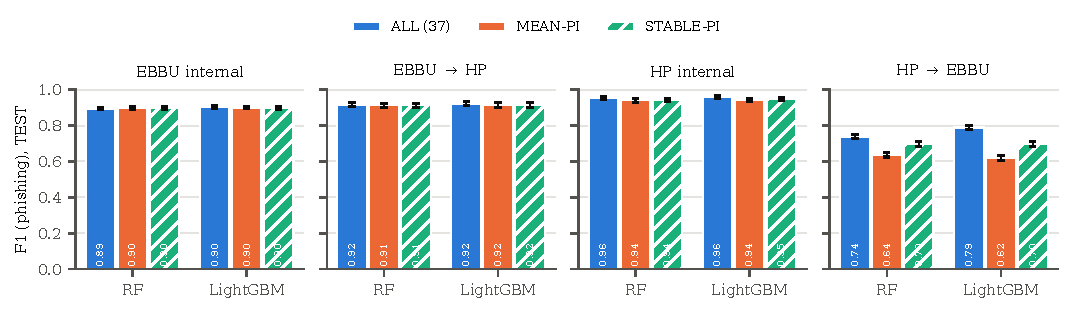
\includegraphics[width=\textwidth]{generated/fig_f1.pdf}
\caption{F1 on TEST for the four evaluation cells (bars: mean of 3 seeds; whiskers: 95\% domain-cluster bootstrap CI). Feature sets: ALL (blue), MEAN-PI (orange), STABLE-PI (green, hatched).}
\label{fig:f1}
\end{figure*}

\subsection{RQ2: stability-based versus mean-importance selection}
Table~\ref{tab:contrasts} lists the four pre-specified contrasts. In EBBU$\rightarrow$HP, differences between STABLE-PI and MEAN-PI are small (RF \res{DeltaABRF} [\res{DeltaLoABRF}, \res{DeltaHiABRF}], LightGBM \res{DeltaABLGBM} [\res{DeltaLoABLGBM}, \res{DeltaHiABLGBM}]) relative to the pre-set practical band. We do not claim statistical equivalence. In HP$\rightarrow$EBBU, the paired differences favour STABLE-PI: \res{DeltaBARF} [\res{DeltaLoBARF}, \res{DeltaHiBARF}] for RF and \res{DeltaBALGBM} [\res{DeltaLoBALGBM}, \res{DeltaHiBALGBM}] for LightGBM; the sign is positive in every seed, although the size varies (Table~\ref{tab:contrasts}). Internally, the observed selector differences are below the practical threshold.

The secondary contrasts temper this result: reduced subsets did not match ALL across both datasets. On HP$\rightarrow$EBBU, the STABLE-PI minus ALL F1 differences are \res{SecBARFSTABLEALL} (RF) and \res{SecBALGBMSTABLEALL} (LightGBM), while MEAN-PI minus ALL gives \res{SecBARFMEANALL} and \res{SecBALGBMMEANALL}. Stability ranking mitigates the loss associated with these compact configurations, without recovering ALL performance. This does not prove that the feature count alone causes the loss; membership and fitted trees also differ. On EBBU$\rightarrow$HP the STABLE-PI minus ALL differences are \res{SecABRFSTABLEALL} and \res{SecABLGBMSTABLEALL}.

\begin{table*}[t]
\caption{Paired domain-cluster bootstrap contrasts of target-TEST F1 (\res{nBoot} replicates; same resampled domains for both arms and all seeds). Top: the four primary contrasts; bottom: secondary cross-dataset contrasts. Per-seed deltas for seeds 17/29/43.}
\label{tab:contrasts}
\centering\scriptsize
\begin{tabular}{lllcccc}
\toprule
Cell & Model & Contrast & $k$ & $\Delta$F1 & 95\% CI & per seed \\
\midrule
A$\rightarrow$B & RF & STABLE vs MEAN (matched $k$) & 16/16/16 vs 16/16/16 & -0.000 & [-0.001, +0.000] & +0.000 +0.002 -0.004 \\
A$\rightarrow$B & LGBM & STABLE vs MEAN (matched $k$) & 16/16/16 vs 16/16/16 & -0.000 & [-0.001, +0.000] & +0.000 -0.002 +0.001 \\
B$\rightarrow$A & RF & STABLE vs MEAN (matched $k$) & 8/8/8 vs 8/8/8 & +0.059 & [+0.051, +0.066] & +0.095 +0.014 +0.066 \\
B$\rightarrow$A & LGBM & STABLE vs MEAN (matched $k$) & 8/8/8 vs 8/8/8 & +0.077 & [+0.069, +0.086] & +0.073 +0.039 +0.120 \\
\midrule
A$\rightarrow$B & RF & STABLE vs ALL & 16/16/16 vs 37/37/37 & -0.004 & [-0.006, -0.003] & -0.001 -0.002 -0.010 \\
A$\rightarrow$B & RF & MEAN vs ALL & 16/16/16 vs 37/37/37 & -0.004 & [-0.005, -0.002] & -0.001 -0.005 -0.006 \\
A$\rightarrow$B & RF & STABLE vs MEAN (budget $k$) & 16/16/16 vs 16/16/16 & -0.000 & [-0.001, +0.000] & +0.000 +0.002 -0.004 \\
A$\rightarrow$B & LGBM & STABLE vs ALL & 16/16/16 vs 37/37/37 & -0.007 & [-0.009, -0.004] & -0.007 -0.007 -0.006 \\
A$\rightarrow$B & LGBM & MEAN vs ALL & 16/16/16 vs 37/37/37 & -0.006 & [-0.009, -0.004] & -0.007 -0.005 -0.007 \\
A$\rightarrow$B & LGBM & STABLE vs MEAN (budget $k$) & 16/16/16 vs 16/16/16 & -0.000 & [-0.001, +0.000] & +0.000 -0.002 +0.001 \\
B$\rightarrow$A & RF & STABLE vs ALL & 8/8/8 vs 37/37/37 & -0.042 & [-0.050, -0.033] & -0.048 -0.027 -0.049 \\
B$\rightarrow$A & RF & MEAN vs ALL & 8/8/8 vs 37/37/37 & -0.100 & [-0.109, -0.092] & -0.143 -0.041 -0.116 \\
B$\rightarrow$A & RF & STABLE vs MEAN (budget $k$) & 8/8/8 vs 8/8/8 & +0.059 & [+0.051, +0.066] & +0.095 +0.014 +0.066 \\
B$\rightarrow$A & LGBM & STABLE vs ALL & 8/8/8 vs 37/37/37 & -0.093 & [-0.101, -0.085] & -0.093 -0.093 -0.093 \\
B$\rightarrow$A & LGBM & MEAN vs ALL & 8/8/8 vs 37/37/37 & -0.170 & [-0.181, -0.159] & -0.166 -0.132 -0.212 \\
B$\rightarrow$A & LGBM & STABLE vs MEAN (budget $k$) & 8/8/8 vs 8/8/8 & +0.077 & [+0.069, +0.086] & +0.073 +0.039 +0.120 \\
\bottomrule
\end{tabular}

\end{table*}

\subsection{RQ3: computational cost}
Table~\ref{tab:cost} and Fig.~\ref{fig:latency} give the latency per URL. For a single URL on one thread, reduced subsets take \res{relLatB1Min}--\res{relLatB1Max} of the end-to-end time of the corresponding ALL model; for batches of 1{,}024 URLs on four threads the ratio is \res{relLatBkMin}--\res{relLatBkMax}. Parsing and feature extraction account for a median of \res{extractShareMedian}\% of single-URL end-to-end time, so pruning features mainly saves extraction work, while tree inference cost depends little on the number of input features.

\begin{table*}[t]
\caption{Cost of the seed-17 model of every configuration (median $\mu$s per URL; ``rel.'' = end-to-end time relative to ALL of the same source and classifier). Hardware: \res{cpu}, \res{ram} GB RAM, Python \res{pyver}.}
\label{tab:cost}
\centering\scriptsize
\begin{tabular}{lllrrrrrrrrr}
\toprule
 & & & & \multicolumn{4}{c}{batch 1, 1 thread ($\mu$s/URL)} & \multicolumn{2}{c}{batch 1024, 4 thr.} & & \\
\cmidrule(lr){5-8}\cmidrule(lr){9-10}
Src & Model & Features & $k$ & extract & predict & e2e & rel. & e2e $\mu$s/URL & rel. & MB & fit s \\
\midrule
A & LGBM & MEAN-PI & 16 & 172 & 821 & 888 & 0.76 & 74.3 & 0.66 & 0.99 & 0.6 \\
A & LGBM & STABLE-PI & 16 & 177 & 598 & 881 & 0.75 & 75.0 & 0.67 & 0.99 & 0.6 \\
A & LGBM & ALL & 37 & 252 & 908 & 1167 & 1.00 & 112.5 & 1.00 & 1.00 & 0.8 \\
A & RF & MEAN-PI & 16 & 131 & 9881 & 9995 & 0.83 & 122.2 & 0.81 & 55.75 & 2.7 \\
A & RF & STABLE-PI & 16 & 112 & 9575 & 10110 & 0.84 & 121.0 & 0.81 & 55.75 & 2.7 \\
A & RF & ALL & 37 & 155 & 10244 & 12094 & 1.00 & 150.3 & 1.00 & 56.45 & 3.1 \\
B & LGBM & MEAN-PI & 8 & 150 & 539 & 772 & 0.93 & 61.0 & 0.55 & 0.99 & 0.6 \\
B & LGBM & STABLE-PI & 8 & 146 & 486 & 721 & 0.87 & 52.6 & 0.47 & 0.99 & 0.5 \\
B & LGBM & ALL & 37 & 228 & 556 & 830 & 1.00 & 111.3 & 1.00 & 1.00 & 0.9 \\
B & RF & MEAN-PI & 8 & 105 & 10316 & 10795 & 1.10 & 152.1 & 1.01 & 45.91 & 1.7 \\
B & RF & STABLE-PI & 8 & 111 & 10704 & 10455 & 1.06 & 92.7 & 0.61 & 44.15 & 1.5 \\
B & RF & ALL & 37 & 150 & 9356 & 9852 & 1.00 & 151.1 & 1.00 & 41.45 & 3.6 \\
\bottomrule
\end{tabular}

\end{table*}

\subsection{RQ4: attributions}
The corrected exploratory explanations pass strict additivity (maximum residual \res{shapAddErr}). The following rankings use these corrected outputs; the original failing outputs remain archived. Numerical consistency does not establish causal attribution or complete explanation fidelity.
SHAP rankings of the same model on source and target TEST samples agree to a Spearman $\rho$ of \res{rhoMin}--\res{rhoMax} (Table~\ref{tab:shap}, Fig.~\ref{fig:shap}); seed-to-seed agreement of the ALL models on the source is at least \res{rhoSeedMin}. Fig.~\ref{fig:pi} shows the permutation-importance evidence from which the subsets were drawn. Because the input distribution changes between cohorts, a different ranking on the target describes \emph{what} the model used there; it is not by itself evidence of an unfaithful explanation, nor of a causal role of a feature.

\begin{table*}[t]
\caption{Exploratory corrected SHAP rank agreement: source vs.\ target TEST ($\rho$, top-10 Jaccard) and across seeds for ALL; top-5 features on the source.}
\label{tab:shap}
\centering\scriptsize
\begin{tabular}{lllcccp{3.2cm}}
\toprule
Dir. & Model & Features & $\rho_{\mathrm{src,tgt}}$ & J$_{10}$ & $\rho_{\mathrm{seeds}}$ & top-5 (source) \\
\midrule
A$\rightarrow$B & LGBM & ALL (37) & 0.99 & 0.82 & 1.00 & \scriptsize F23 F09 F30 F06 F03 \\
A$\rightarrow$B & LGBM & STABLE-PI & 0.88 & 0.82 & -- & \scriptsize F23 F09 F03 F06 F30 \\
A$\rightarrow$B & RF & ALL (37) & 0.97 & 0.82 & 1.00 & \scriptsize F23 F09 F30 F07 F03 \\
A$\rightarrow$B & RF & STABLE-PI & 0.81 & 0.82 & -- & \scriptsize F23 F09 F03 F30 F07 \\
B$\rightarrow$A & LGBM & ALL (37) & 0.96 & 0.82 & 1.00 & \scriptsize F02 F23 F06 F03 F22 \\
B$\rightarrow$A & LGBM & STABLE-PI & 0.98 & 1.00 & -- & \scriptsize F02 F23 F03 F06 F21 \\
B$\rightarrow$A & RF & ALL (37) & 0.95 & 0.82 & 1.00 & \scriptsize F02 F23 F06 F01 F03 \\
B$\rightarrow$A & RF & STABLE-PI & 0.98 & 1.00 & -- & \scriptsize F02 F23 F06 F03 F21 \\
\bottomrule
\end{tabular}

\end{table*}

\begin{figure*}[t]
\centering
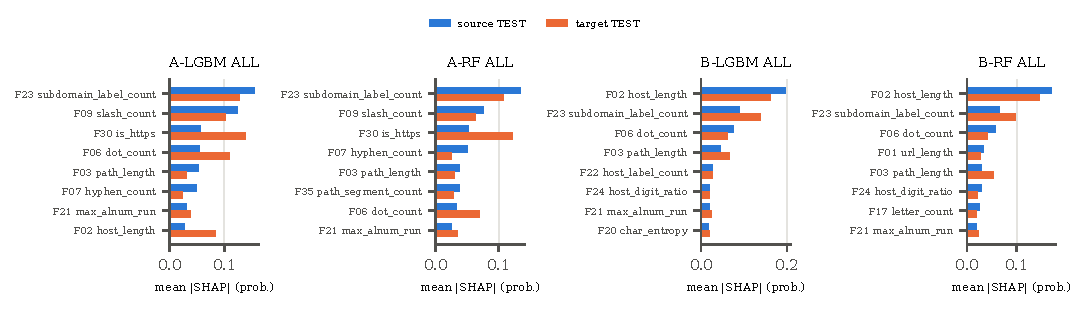
\includegraphics[width=\textwidth]{generated/fig_shap.pdf}
\caption{Exploratory corrected mean $|$SHAP$|$ (probability scale) of the eight most important features of the seed-17 ALL models on source TEST (blue) and target TEST (orange).}
\label{fig:shap}
\end{figure*}

\begin{figure*}[t]
\centering
\begin{minipage}[t]{0.48\textwidth}
\centering\vspace{0pt}
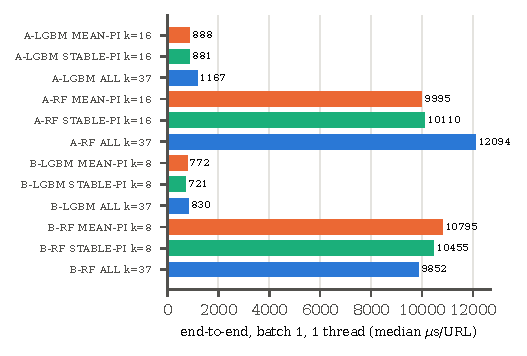
\includegraphics[width=\linewidth]{generated/fig_latency.pdf}
\caption{End-to-end latency for a single URL on one thread (seed-17 models).}
\label{fig:latency}
\end{minipage}\hfill
\begin{minipage}[t]{0.48\textwidth}
\centering\vspace{0pt}
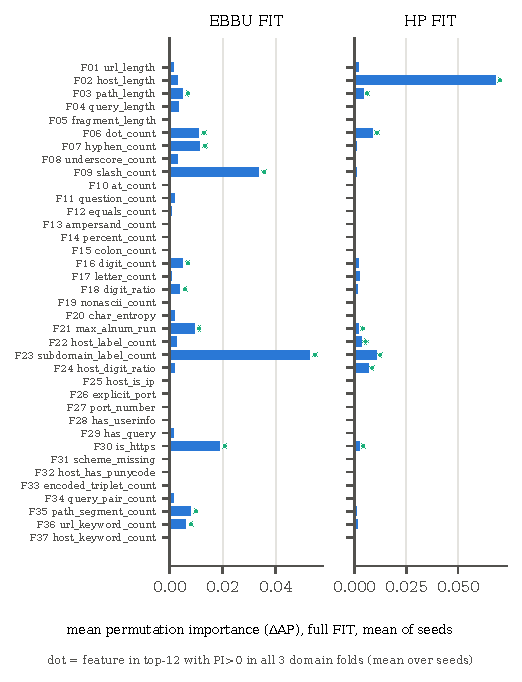
\includegraphics[width=\linewidth]{generated/fig_pi.pdf}
\caption{Permutation importance on full FIT (mean over folds and seeds). Dots mark features that are in the top 12 with positive PI in all three domain folds.}
\label{fig:pi}
\end{minipage}
\end{figure*}
